\documentclass[11pt]{article}
\usepackage[utf8]{inputenc}
\usepackage{hyperref}
\usepackage{biblatex}
\usepackage{graphicx}

\title{\textbf{NSF Research Proposal}}
\author{Amartya Dutta}
\date{}


\usepackage[letterpaper, margin=1in]{geometry}
\addbibresource{ref.bib}

\begin{document}
\clearpage\maketitle
\thispagestyle{empty}
\section{Project summary}
Semantic segmentation is a computer vision task that involves assigning a class label to every pixel in an image. The goal is to understand the image at the pixel level, partitioning it into semantically meaningful regions corresponding to different objects or structures. This enables a more detailed and granular understanding of the scene, as opposed to traditional object recognition methods that identify the presence of objects without capturing their spatial distribution. Weakly supervised semantic segmentation on the other hand refers to learning segmentation models from data with limited or incomplete annotations. In contrast to fully supervised methods that require dense pixel-wise annotations, weakly supervised approaches rely on weaker forms of supervision, such as image-level labels, bounding boxes, or scribbles. The main motivation behind weakly supervised semantic segmentation is to reduce the reliance on expensive and time-consuming pixel-level annotations, which can be a significant bottleneck in developing segmentation models. \newline
Weakly supervised semantic segmentation offers several advantages compared to fully supervised methods:
\begin{itemize}
\item \textbf{Reduced annotation effort}: Obtaining pixel-level annotations for large datasets is labor-intensive and costly. Weakly supervised methods alleviate this burden by leveraging weaker, more easily obtainable forms of supervision.
\item \textbf{Scalability}: The reduced annotation requirements enable the application of semantic segmentation to larger datasets and domains where dense annotations are impractical or unavailable.
\item \textbf{Robustness}: Learning from weaker supervision can encourage the model to capture more generalizable patterns and representations, potentially leading to better performance in the presence of domain shifts or novel object classes.
\end{itemize}
The challenge lies in designing algorithms that can effectively leverage limited annotations to produce accurate segmentation. The proposed research aims to develop novel weakly supervised segmentation methods that address these challenges and achieve high performance while benefiting from the advantages of weak supervision.

\section{Intellectual merits}
The intellectual merits of the research on weakly-supervised semantic segmentation are numerous, as it aims to address fundamental challenges in computer vision and develop innovative methods that can significantly improve segmentation performance with limited annotations. Some of the key intellectual merits include:
\begin{itemize}
    \item \textbf{Advancing the state-of-the-art}: Developing novel weakly supervised semantic segmentation algorithms can significantly improve performance, efficiency, and scalability compared to existing methods. This can push the boundaries of current knowledge and understanding in the field of computer vision.
    \item \textbf{Theoretical insights}: Investigating weakly supervised semantic segmentation can provide new theoretical insights into the learning processes and generalization capabilities of such models. This can help establish a deeper understanding of the underlying principles that govern weak supervision and its implications for model performance.
     \item \textbf{Algorithmic innovations}: Proposing new weakly supervised methods can lead to the development of innovative techniques, architectures, and learning strategies. These advances can have implications beyond semantic segmentation and can be adapted for other computer vision tasks or even other domains that rely on machine learning.
     \item \textbf{Data efficiency}: One of the main goals of weakly supervised semantic segmentation is to make better use of limited annotations. Novel research in this area can lead to more efficient algorithms that can learn from smaller amounts of labeled data, reducing the dependency on expensive and labor-intensive pixel-level annotations.
     \item \textbf{Cross-domain applicability}: Developing efficient weakly supervised semantic segmentation methods can have a broad impact on various domains, such as autonomous vehicles, remote sensing, and healthcare, where semantic segmentation is a critical component. Improved methods in this area can lead to better performance and more robust solutions in these application domains.

\end{itemize}
Overall, conducting research on weakly-supervised semantic segmentation can significantly advance our understanding of the learning process, contribute to the development of new techniques, and have wide-ranging implications for both the field of computer vision and numerous real-world applications.
\section{Broader impacts}
The research on weakly-supervised semantic segmentation can have broader impacts across multiple domains that rely on semantic segmentation, as it aims to reduce annotation effort, increase data efficiency, and enable scalable solutions. Some of the key broader impacts include:
\begin{itemize}
    \item \textbf{Autonomous vehicles}: Improved weakly supervised semantic segmentation methods can enhance the perception capabilities of self-driving cars by enabling a more accurate understanding of their surroundings. This can lead to safer and more reliable autonomous transportation systems.
    \item \textbf{Remote sensing}: Efficient weakly supervised learning techniques can facilitate the analysis of satellite and aerial imagery, allowing for more accurate land use classification, environmental monitoring, and disaster management. This can help in making better-informed decisions for sustainable land use and resource allocation.
     \item \textbf{Healthcare}: Better semantic segmentation algorithms can contribute to the analysis of medical images, such as MRIs, CT scans, and X-rays, improving the accuracy and speed of diagnosis, treatment planning, and monitoring of diseases.
    \item \textbf{Robotics}: In the field of robotics, efficient weakly supervised semantic segmentation can help robots better understand and interact with their environment, enabling tasks such as navigation, manipulation, and object recognition with less reliance on dense annotations.
    \item \textbf{Agriculture}: Advanced weakly supervised semantic segmentation methods can be used to analyze drone or satellite imagery for precision agriculture, enabling farmers to monitor crop health, detect diseases and pests, and optimize irrigation and fertilizer management.
    \item \textbf{Conservation and ecology}: Improved semantic segmentation can aid in monitoring wildlife populations, habitat conditions, and human-induced changes to ecosystems, providing valuable data for conservation planning and ecological research.
    
\end{itemize}
By advancing the state-of-the-art in weakly supervised semantic segmentation, the proposed research can benefit a wide range of applications across various domains, resulting in positive impacts on society, the economy, and the environment.

\section{Related work}
Recently a large body of work has focused on providing explanations of the model outputs which can potentially satisfy regulatory experiments, help practitioners debug their model, and identify unintended bias in the model. This area of model explainability techniques can be categorized into two broad categories: (1) activation map-based methods \cite{zhou2016learning, selvaraju2016grad}, (2) attribution map-based methods \cite{simonyan2013deep, baehrens2010explain}.  \newline
\textbf{Activation maps} are feature maps from the last layer of CNNs which show regions in an image that is most responsible for the final prediction of the network. The activations are aggregated to generate a heatmap, highlighting the regions in the image with the highest activations. One of the most popular activation map-based methods is Class Activation Maps (CAMs) \cite{zhou2016learning}, where the activation map of the last CNN layer is combined with weights of the Global Average Pooling (GAP) layer to generate the visual explanations. Gradient-weighted Class Activation Mapping (Grad-CAM) \cite{selvaraju2016grad} is an extension of CAM that uses gradient information to improve the localization accuracy of the generated heatmaps. \textbf{Attribution maps} on the other hand are a form of interpretability technique that attempts to assign a score to each pixel in an image, representing its contribution to the final prediction of the network. There are various methods to compute attribution maps such as gradient-based methods. Gradient-based saliency map methods \cite{simonyan2013deep,baehrens2010explain} is the most common example of such a category, where the attribution map is generated by computing the gradient of the target class score w.r.t. the input image. The gradient quantifies how much change in the input pixel values corresponds to the change in target class scores. \newline
While Class Activation Maps (CAM) are good at highlighting discriminative regions (DR) of an image (i.e., regions that contribute significantly to the classifier’s decision), CAMs are known to disregard regions of the target object class that do not contribute to the classifier’s prediction, termed non-discriminative regions (NDR). This is because Class Activation Maps (CAMs) are essentially \textbf{activation maps} generated by the last convolutional neural network (CNN) layer, which are integrated with the weights of the final fully-connected layer. It has been shown that the final layer feature maps only contain information relevant to classification, a phenomenon called \textit{information bottleneck} \cite{lee2021reducing}. The RIB \cite{lee2021reducing} demonstrates that an information bottleneck occurs in later layers as only the task-relevant information is passed to the output. As a result, CAMs that are computed at the last layer have sparse coverage of the target object. Thus, CAMs are biased towards mostly finding DR while missing the NDR of the target object, which is equally important for the purpose of segmentation. A number of WS3 solutions thus require further processing of the CAM outputs to recover NDR for high segmentation accuracy \cite{li2018tell, hou2018self}. \newline
In contrast to activation maps, \textbf{attribution maps} provide an alternative approach for assigning a score to every pixel based on its contribution to the final neural network prediction. The most commonly used attribution map is the gradient-based Saliency Maps \cite{simonyan2013deep}. The basic idea of saliency is to calculate the gradient of the target class score with respect to every pixel in the input image. Attribution maps are fundamentally distinct from the activation maps obtained from the last layer of CNN models. However, despite the frequent use of attribution maps for interpretability purposes, their utility in WS3 has not yet been fully explored. \newline
While these approaches have shown promising results, there remains room for improvement in terms of accuracy, efficiency, and scalability, which motivates the proposed research.
\section{Proposed research}
The proposed research for weakly supervised semantic segmentation aims to develop novel algorithms utilizing Saliency Maps that can effectively leverage limited annotations to achieve high performance and improve efficiency and scalability. The proposed research objectives can be outlined as follows:
\begin{itemize}
\item Design and develop novel weakly supervised semantic segmentation algorithms based on Saliency Maps that can effectively leverage limited annotations for accurate and efficient segmentation. This will involve exploring new architectures and loss functions that better capture the entirety of an object and thus better utilizes weak supervision in the learning process.
\item Investigate how to combine different sources of weak supervision (e.g., image-level labels, sparse annotations) and explore the potential synergies for improved performance. This may involve developing methods that can fuse weak supervision cues and propagate information across different levels of annotation granularity.
\item Analyze the generalization capabilities of Saliency Map-based weakly supervised models as compared to CAM to provide insights into the strengths and limitations of different weak supervision strategies. This will help understand the trade-offs between annotation effort and model performance and can guide the development of more effective weakly supervised algorithms.
\item Propose practical and efficient annotation strategies to guide the collection of limited but informative labels for training weakly supervised models. This may involve designing active learning approaches or other sampling techniques that can identify the most informative examples for annotation, thus reducing the overall annotation effort required.
\item Evaluate and benchmark the developed weakly supervised semantic segmentation algorithms on various public datasets and real-world applications to assess their performance, efficiency, and scalability. This will involve rigorous empirical evaluation and comparisons with state-of-the-art methods, helping to establish the effectiveness of the proposed research.
\end{itemize}
By pursuing these research objectives, the proposed study aims to make significant advancements in weakly supervised semantic segmentation, benefiting a wide range of applications across multiple domains.
\section{Research Timeline}
\begin{figure}[h!]
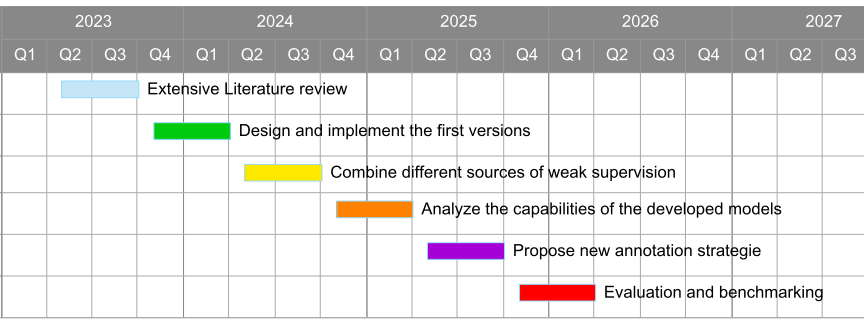
\includegraphics[scale=0.75]{Gantt.png}
\centering
\caption{Gantt Chart Showing the Timeline of Proposed Research}
\label{chart}
\end{figure}

The proposed research will be carried out over a period of three years as shown in Fig. \ref{chart}. Each Q followed by a number in the chart refers to the Quarter Number of the year. The set of tasks can be divided into six main stages as follows:
\begin{itemize}
\item \textbf{Months 1-6}: Conduct a comprehensive literature review of existing weakly supervised semantic segmentation methods and identify current gaps and limitations. Develop initial ideas and hypotheses for novel algorithms.

\item \textbf{Months 7-12}: Design and implement the first version of the proposed weakly supervised semantic segmentation algorithms. Perform initial experiments and evaluate their performance against current state-of-the-art methods. Identify areas for further improvement.

\item \textbf{Months 13-18}: Explore techniques to combine different sources of weak supervision and develop novel algorithms to exploit their synergies. Investigate the use of additional cues, such as depth, context, or motion, to improve segmentation performance.

\item \textbf{Months 19-24}: Analyze the generalization capabilities of the developed models and investigate the strengths and limitations of different weak supervision strategies. Based on these insights, refine the proposed algorithms to enhance their generalization performance.

\item \textbf{Months 25-30}: Propose and evaluate practical annotation strategies that guide the collection of limited but informative labels for training weakly supervised models. Assess the effectiveness of these strategies in terms of annotation effort and model performance.

\item \textbf{Months 31-36}: Perform extensive evaluation and benchmarking of the final weakly supervised semantic segmentation algorithms on various public datasets and real-world applications. Prepare publications and disseminate the results to the research community.

\end{itemize}
The proposed research is expected to yield significant advancements in weakly supervised semantic segmentation, benefiting a wide range of applications across multiple domains.
\newpage
\printbibliography
\end{document}